%
% Author: Riccardo Orizio
% Date: Fri 31 Aug 2018
% Description: Presentation for Lero Symposium on September 4
%

\documentclass{beamer}

\usepackage[utf8]{inputenc}
\usepackage{graphicx}
\usepackage{amsmath}

\graphicspath{ {./Images/} }

% Style properties
\usetheme{Warsaw}
\usefonttheme{structuresmallcapsserif}
\usefonttheme{professionalfonts}
\usecolortheme{seahorse}

\setbeamertemplate{caption}{\raggedright\insertcaption\par}

% Defining a unique space modifier, mostly used in the itemize environment
\def\itemizespace{\vspace{7mm}}

% Title page information
\title[Lero Symposium 2018]{Improving security and resilience of Cyber Physical Systems}
\author[Provan G., Orizio R.]{Riccardo Orizio \\ \small{Prof. Gregory Provan}}
\institute[UCC]
{
	Department of Computer Science\\
	\vspace{1mm}
	University College Cork\\
}
\date[2018]{04 September 2018}
\titlegraphic
{
	
\includegraphics[width=0.15\textwidth]{logo_lero.jpg}
	\hspace{0.2\textwidth}
	
\includegraphics[width=0.15\textwidth]{logo_sfi.jpg}
	\hspace{0.2\textwidth}
	
\includegraphics[width=0.15\textwidth]{logo_ucc.png}
}


\begin{document}

\begin{frame}
	\titlepage
\end{frame}

% Table of contents?

%%%%%%%%%%%%%%%%%%%%%%%%%%%%%%%%%%%%%%%%%%%%%%%%%%%%%%%%%%%%%%%%%%%%%%%%%%%%%%

\section{Research Question}

\subsection{General Problem}
\begin{frame}{Cyber Physical Systems}
	\begin{itemize}[<+->]
		\item[] Cyber Physical Systems are made of three main parts:
			\begin{itemize}
				\item[-]<1-> physical processes;
				\item[-]<1-> computational resources;
				\item[-]<1-> communication infrastructures.
			\end{itemize}

		\itemizespace%

		\item[] Most real systems can be represented with this structure, i.e.,
			transportation networks, electrical and gas distribution systems,
			water treatment plants, etc...

		\itemizespace%

		\item[] These systems have to be reliable at all time and in all
			circumstances.
			Especially when anomalies occur, regardless of their nature, the
			system needs to react and overcome the issue.

	\end{itemize}
\end{frame}

\begin{frame}{Stuxnet: real life scenario threat}
	\begin{itemize}[<+->]
		\item[] A malicious computer worm created in 2005 by American/Israeli
			governments to damage Iran's nuclear program;

		\itemizespace%

		\item[] Target SCADA infrastructure and PLC systems to physically
			compromise their centrifuges and reduce their overall productivity;

		\itemizespace%

		\item[] Discovered only in 2010 because it spread itself too far.
	\end{itemize}
\end{frame}

\subsection{Our contribution}
\begin{frame}{Question}
	\begin{itemize}[<+->]
		\item[] Can we create a tool that can help these systems in detecting,
			identifying and correcting an anomaly whenever one would occur?
		
		\itemizespace%

		\item[] Can it be used for real time systems?

		\itemizespace%
			
		\item[] And can it be an all purpose tool used on a wide variety of
			different systems?
	\end{itemize}
\end{frame}

%%%%%%%%%%%%%%%%%%%%%%%%%%%%%%%%%%%%%%%%%%%%%%%%%%%%%%%%%%%%%%%%%%%%%%%%%%%%%%

\section{Research Method}
\begin{frame}{Research method}
	\begin{itemize}[<+->]
		\item[] Experimental based approach;

		\itemizespace%

		\item[] Currently experimenting on simulations of the three tanks model
			and its variations.
			\vspace{2mm}
			\begin{figure}
				\centering
				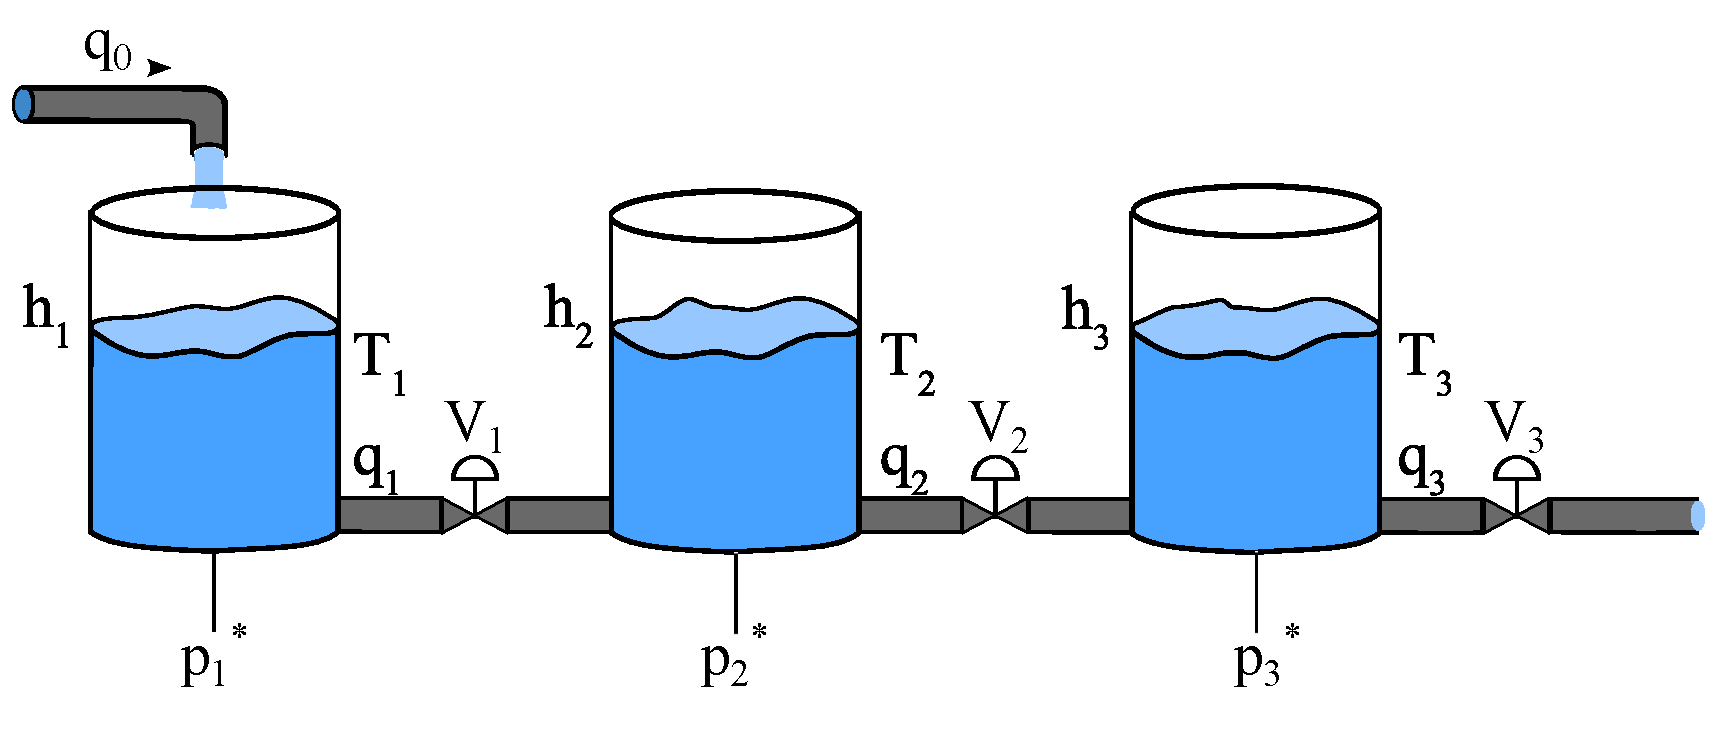
\includegraphics[width=0.6\textwidth]{3-tanks.pdf}
			\end{figure}
	\end{itemize}
\end{frame}

%%%%%%%%%%%%%%%%%%%%%%%%%%%%%%%%%%%%%%%%%%%%%%%%%%%%%%%%%%%%%%%%%%%%%%%%%%%%%%

\section{Summary of Research to date}

\subsection{Model based approach}
\begin{frame}{Model based approach}
	\begin{itemize}[<+->]
		\item[] A CPS model can operate in different behaviours, called modes:
			\[
				Modes:	\begin{cases}
							y_{m_1} = g_1(x)	\\
							...					\\
							y_{m_i} = g_i(x)	\\
						\end{cases}
			\]

		\itemizespace%

		\item[] Diagnosis is an inverse inference on the modes set: 
			$$ x = g^{-1}_{i}(y_i) $$ 
			In most cases $ g( \cdot ) $ is non-linear.

		\itemizespace%

		\item[] Multi modes simultaneously active will increase exponentially
			the inverse inference computation.
    \end{itemize}
\end{frame}

\subsection{Residual study approach}
\begin{frame}{Residual study approach}
	\begin{itemize}[<+->]
		\item[] Study the system only from the data provided from their sensors;

		\itemizespace%

		\item[] Residual: $ r_i = y_{real_i} - y_{nominal_i} \ \forall i \in
			\{sensors\}$;

		\itemizespace%

		\item[] Anomaly identification activated iff $ r > \delta $, studying
			the systems' sensors data and their first derivative;

		\itemizespace%

		\item[] Results:
			\begin{itemize}
				\item[-]<3-> Primitive and basic approach;
				\item[-]<3-> Able to recognize some simple attacks;
				\item[-]<3-> Plenty of false positives when the anomalies
					affects the internal components of the system.
			\end{itemize}

	\end{itemize}
\end{frame}

\begin{frame}{Residual study results}
	\begin{columns}
		\begin{column}{0.45\textwidth}
			\begin{figure}
				\centering
				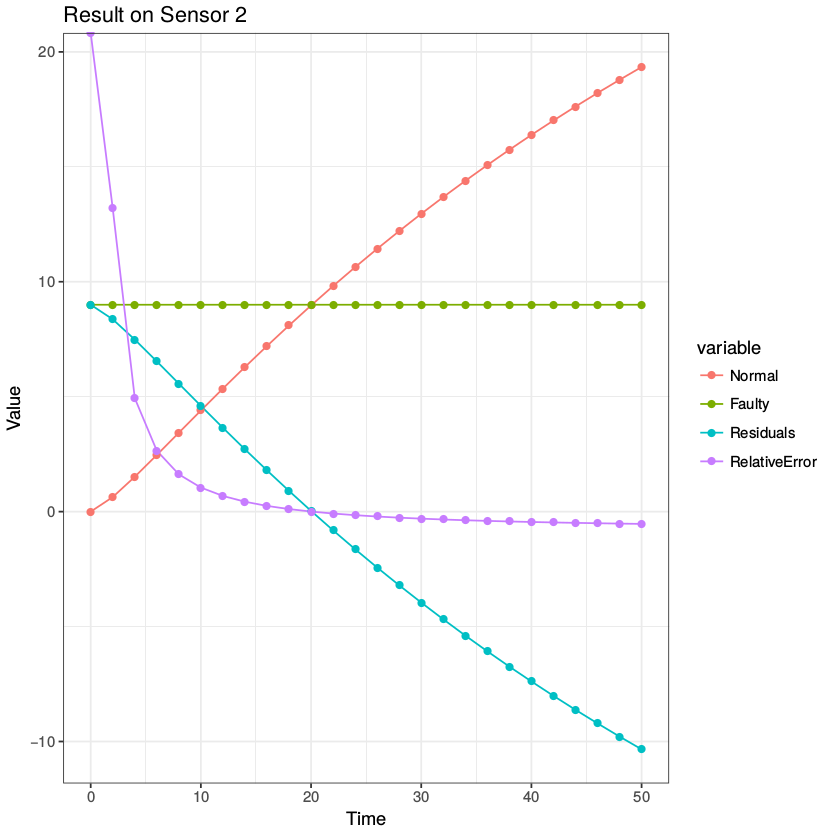
\includegraphics[width=0.9\textwidth]{attack_sensor2_2.png}
				\caption{A sensor of the system is attacked. Identifiable
				through: $ \dot{y}_k=-\dot{r}_k $.}
			\end{figure}
		\end{column}

		\begin{column}{0.45\textwidth}
			\begin{figure}
				\centering
				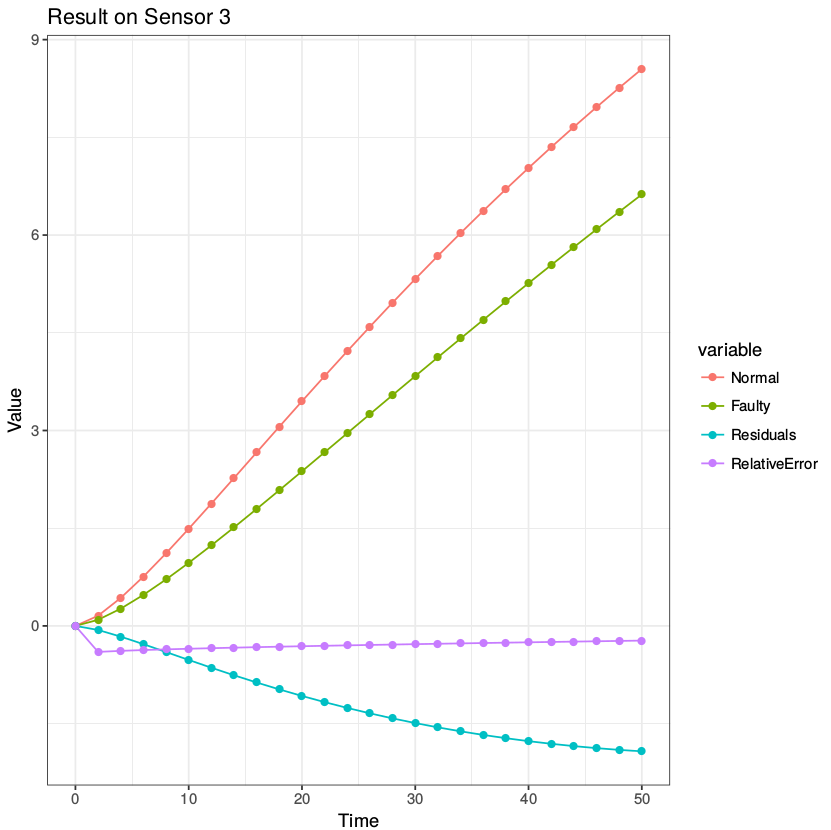
\includegraphics[width=0.9\textwidth]{attack_valve.png}
				\caption{Synergies of the system make it harder to identify the
				anomaly.}
			\end{figure}
		\end{column}
	\end{columns}
\end{frame}

\subsection{Algebraic approach}
\begin{frame}{Algebraic approach}
	\begin{description}[<+->]
		\item[Basic:] Extend the sensors data study to higher order derivatives
			looking for particular patterns that could identify the anomalies;

		\itemizespace%

		\item[Improved:] Use the patterns to find anomalies masked from other
			anomalies.

	\end{description}
\end{frame}
\begin{frame}{Example}
	\begin{figure}
		\centering
		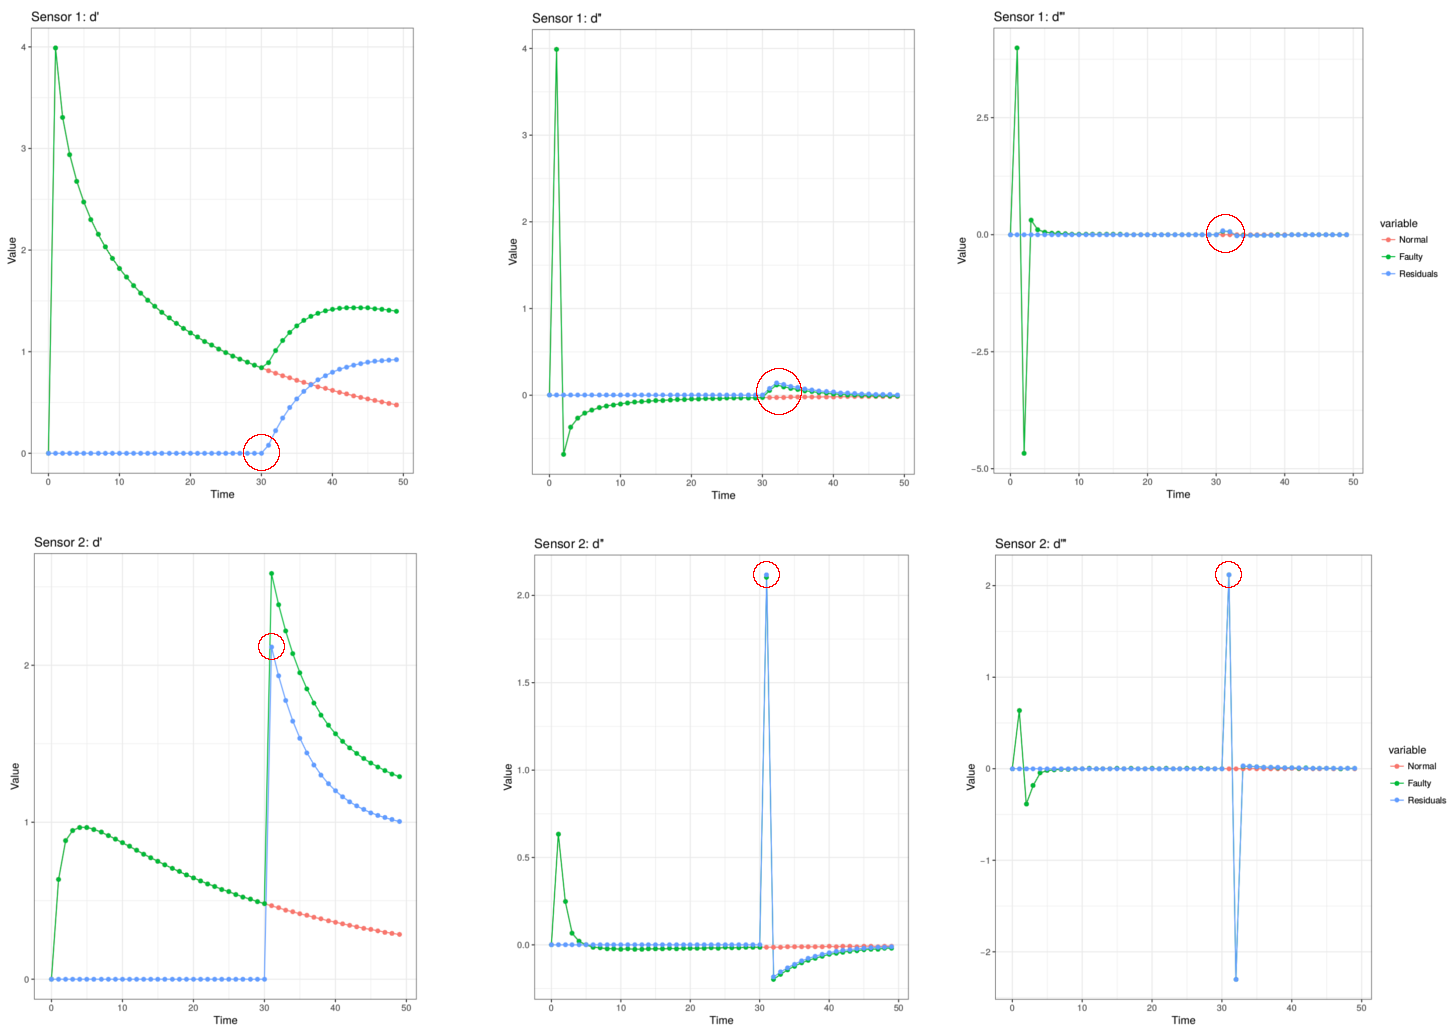
\includegraphics[width=0.7\textwidth]{attack_peak_circled.png}
		\caption{Peculiar pattern of an actuator attack on the system and its
		side effects.}
	\end{figure}
\end{frame}

\subsection{Data driven approach}
\begin{frame}{Data driven approach}
	\begin{itemize}[<+->]
		\item[] Can we identify anomaly patterns automatically?

		\itemizespace%

		\item[] Classification of the anomalies' data behaviours through SVM,
			LSTM and HMM.
	\end{itemize}
\end{frame}

\subsection{Results}
\begin{frame}{Results compared}
	\begin{figure}
		\centering
		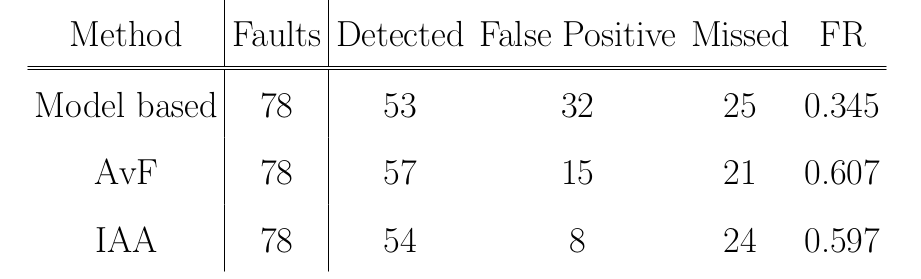
\includegraphics[width=0.8\textwidth]{comparison_results.png}
		\caption{Comparing the results of all the approaches studied to this
		point. The algebraic approach seems the best so far.}
	\end{figure}
\end{frame}
\begin{frame}{Attack or fault distinction: a novel method}
	\begin{figure}
		\centering
		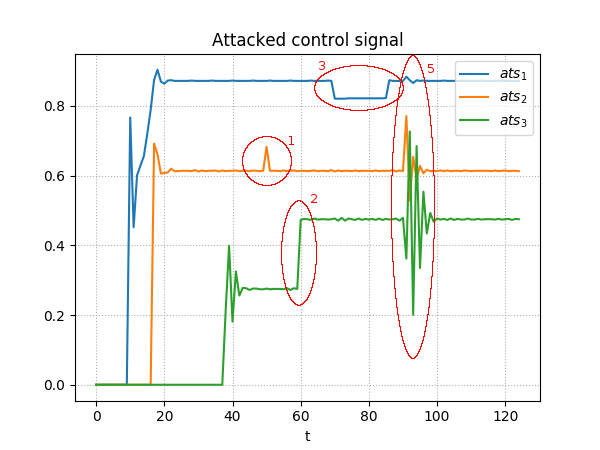
\includegraphics[width=0.36\textwidth]{attacked_signal_improved.png}
		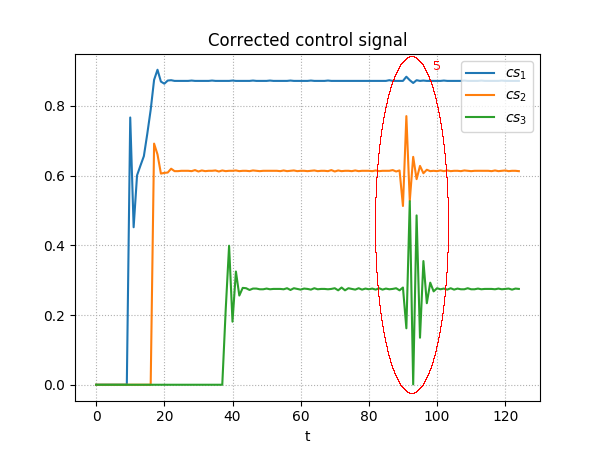
\includegraphics[width=0.36\textwidth]{control_signal_improved.png}
		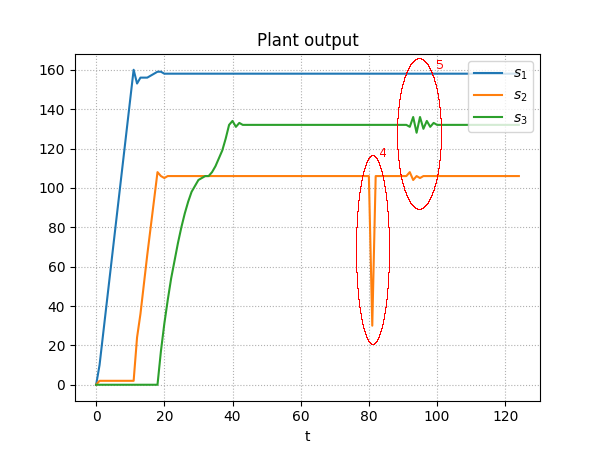
\includegraphics[width=0.36\textwidth]{sensors_improved.png}
		\caption{Using the system to understand if the control signal has been
		tampered.}
	\end{figure}
\end{frame}


%%%%%%%%%%%%%%%%%%%%%%%%%%%%%%%%%%%%%%%%%%%%%%%%%%%%%%%%%%%%%%%%%%%%%%%%%%%%%%

\section{Plan for next 12 months}
\begin{frame}{Future}
	\begin{itemize}
		\item[] Identify a small set of the best approaches for the diagnosis
			process, focusing mainly on data driven ones;

		\itemizespace%

		\item[] Increase the diagnosis efficacy combining different approaches;

		\itemizespace%

		\item[] Extend the tests to real systems;

		\itemizespace%

		\item[] Create a standalone diagnosis tool based on our method.
		
	\end{itemize}
\end{frame}

%%%%%%%%%%%%%%%%%%%%%%%%%%%%%%%%%%%%%%%%%%%%%%%%%%%%%%%%%%%%%%%%%%%%%%%%%%%%%%

\section{}
\begin{frame}
	\begin{figure}
		\centering
		
\includegraphics[height=0.5\textheight]{thank-you.jpg}
	\end{figure}
\end{frame}

\end{document}

